\documentclass[conference]{IEEEtran}
\IEEEoverridecommandlockouts
\usepackage{cite}
\usepackage{amsmath,amssymb,amsfonts}
\usepackage{algorithmic}
\usepackage{graphicx}
\usepackage{textcomp}
\usepackage[table]{xcolor}
\usepackage{booktabs}
\usepackage{multirow}
\usepackage{url}

\def\BibTeX{{\rm B\kern-.05em{\sc i\kern-.025em b}\kern-.08em
    T\kern-.1667em\lower.7ex\hbox{E}\kern-.125emX}}

\begin{document}

\title{An Explainable Deep Learning Framework for Ordinal Crop Disease Severity Grading and Identification in Paddy and Arecanut}

\author{
\IEEEauthorblockN{Sahith R}
\IEEEauthorblockA{\textit{Department of Computer Science} \\
\textit{Dr. NSAM First Grade College Nitte} \\
Karkala, India \\
sahithk64@gmail.com}
}

\maketitle

\begin{abstract}
Accurate, automated estimation of crop disease severity and categorical identification is critical for precision agriculture. While categorical disease classification has advanced rapidly, ordinal severity grading remains constrained by annotation scarcity and, as this paper demonstrates, by split-leakage that is easy to overlook in small, field-collected agricultural datasets. We present an explainable deep learning framework for joint disease identification and ordinal severity grading, grounded in the Horsfall--Barratt scale, evaluated on the public Paddy Doctor benchmark ($N=10{,}053$) and an Arecanut field dataset ($N=2{,}661$). Severity labels are derived automatically from a dual-color-space lesion-ratio pipeline. On Paddy, our ResNet-18 disease classifier reaches 96.04\% accuracy, and Conditional Ordinal Regression for Neural networks (CORN) achieves a quadratic weighted kappa (QWK) of 0.9390 on the full test set, falling to 0.7055 on a lesion-only, near-duplicate-free subset once class-determined categories and near-duplicate test images are removed. On Arecanut, we found that naive split construction -- including a construction we ourselves built and initially trusted -- left 70--80\% of test images sharing photographic session, camera-burst, or soft perceptual-hash overlap with training data across every split we built, inflating QWK from a genuine $0.70$ to an apparent $0.87$--$0.93$. On the largest fully independent, audited subset we could establish ($N=111$), CORN achieves $0.6998 \pm 0.0449$ QWK versus $0.6280 \pm 0.1039$ for a Softmax baseline; the wide, overlapping confidence intervals mean this difference is not statistically distinguishable at the available sample size. A class-identity baseline that ignores the image and predicts each image's most common training-set grade for its disease class matches or exceeds several trained models on Arecanut, showing that headline severity metrics on class-imbalanced field datasets can be dominated by disease recognition rather than severity assessment. An explainability audit using Grad-CAM and Grad-CAM++ finds diseased-tissue pointing-game accuracy of only 5--14\%, and confirms a strong linear confound between Grad-CAM/lesion-mask IoU and raw lesion area ($R^2=0.82$). We report these results, including the negative and null findings, as evidence for what this class of pipeline can and cannot currently support.
\end{abstract}

\begin{IEEEkeywords}
Arecanut, crop disease severity, Conditional Ordinal Regression for Neural networks (CORN), explainable artificial intelligence (XAI), Grad-CAM, Horsfall--Barratt scale, ordinal classification, Paddy Doctor, split-leakage audit.
\end{IEEEkeywords}

\section*{Note to Practitioners}
This work addresses automated plant disease severity assessment for agricultural extension officers and smallholder farmers. Our audit highlights two practical cautions for field deployment: first, model attention frequently does not land on diseased tissue itself, requiring visual oversight before taking chemical treatment decisions; second, standard train/test splits silently inflate performance metrics through photographic session overlap, necessitating multi-criteria perceptual hash auditing on small agricultural datasets.

\section{Introduction}
Quantifying plant disease severity -- the proportion of diseased tissue relative to total organ surface area -- is essential for targeted agricultural management. While deep neural networks have achieved high accuracy in categorical disease identification \cite{petchiammal2023paddy, mohanty2016using, ferentinos2018deep}, nominal classification treats all misclassification errors equally and fails to model continuous intra-class disease progression \cite{horsfall1945fungicides, bock2022plant}. Existing severity assessment approaches in cash crops such as Arecanut often rely on expensive spectroscopic equipment ($>\$10{,}000$) \cite{kushalatha2024spectroscopy}, while RGB-only models risk exploiting background artifacts rather than true pathological lesions \cite{selvaraju2017grad}.

A further, less-discussed risk in small agricultural datasets is split leakage: sequential burst photographs or near-duplicate crops of the same physical plant appearing in both the training and test partitions. This risk is amplified when public datasets are supplemented with external sources collected during the same photography campaign. In the course of this work, we discovered this risk firsthand: a split we constructed and initially validated using parent-plant and perceptual-hash deduplication still allowed 70--80\% of test images to share session-level similarity with training images, inflating our own reported Arecanut severity QWK from a genuine $\approx 0.70$ to an apparent $0.87$--$0.93$ before a finer-grained audit caught it. We report this discovery, and the audit methodology that uncovered it, as a central contribution of this paper, since we believe the same failure mode likely affects other small, field-collected agricultural benchmarks that have not been checked this closely.

The key contributions of this paper are:
\begin{itemize}
    \item \textbf{A weakly supervised labeling pipeline}: an adaptive dual-color-space (HSV/Lab) segmentation pipeline that derives continuous lesion-area ratios and maps them to four ordinal Horsfall--Barratt severity grades, removing the need for manual pixel annotation.
    \item \textbf{A multi-criteria leakage audit that found and corrected our own split-construction errors}: combining base-photo lineage matching, camera-burst timestamp windows, and soft perceptual hashing (Hamming distance 9--16, not just exact-duplicate thresholds), we show this wider check is necessary -- narrower checks using only exact-duplicate pHash or burst-window grouping reported 0\% leakage on splits that this wider check found to be 70--80\% contaminated.
    \item \textbf{Evidence that headline severity metrics on Arecanut are confounded with disease identity}: a trivial class-mode baseline, which ignores the image entirely, matches or exceeds trained severity models on several evaluation subsets, showing that apparent severity-grading skill can be an artifact of disease recognition.
    \item \textbf{Statistically audited ordinal-vs-nominal comparison}: CORN and Softmax are compared via McNemar's test and cluster-grouped bootstrap confidence intervals on both crops; we find no statistically significant exact-accuracy difference between the two losses on either crop, consistent with the theoretical expectation that ordinal losses primarily bound rank-distance error rather than improve top-1 accuracy.
    \item \textbf{A dual-method explainability audit}: Grad-CAM and Grad-CAM++ pointing-game analysis converges on the same conclusion -- the model's attention is only weakly grounded in true lesion tissue for most disease classes.
\end{itemize}

\begin{figure}[t]
\centering
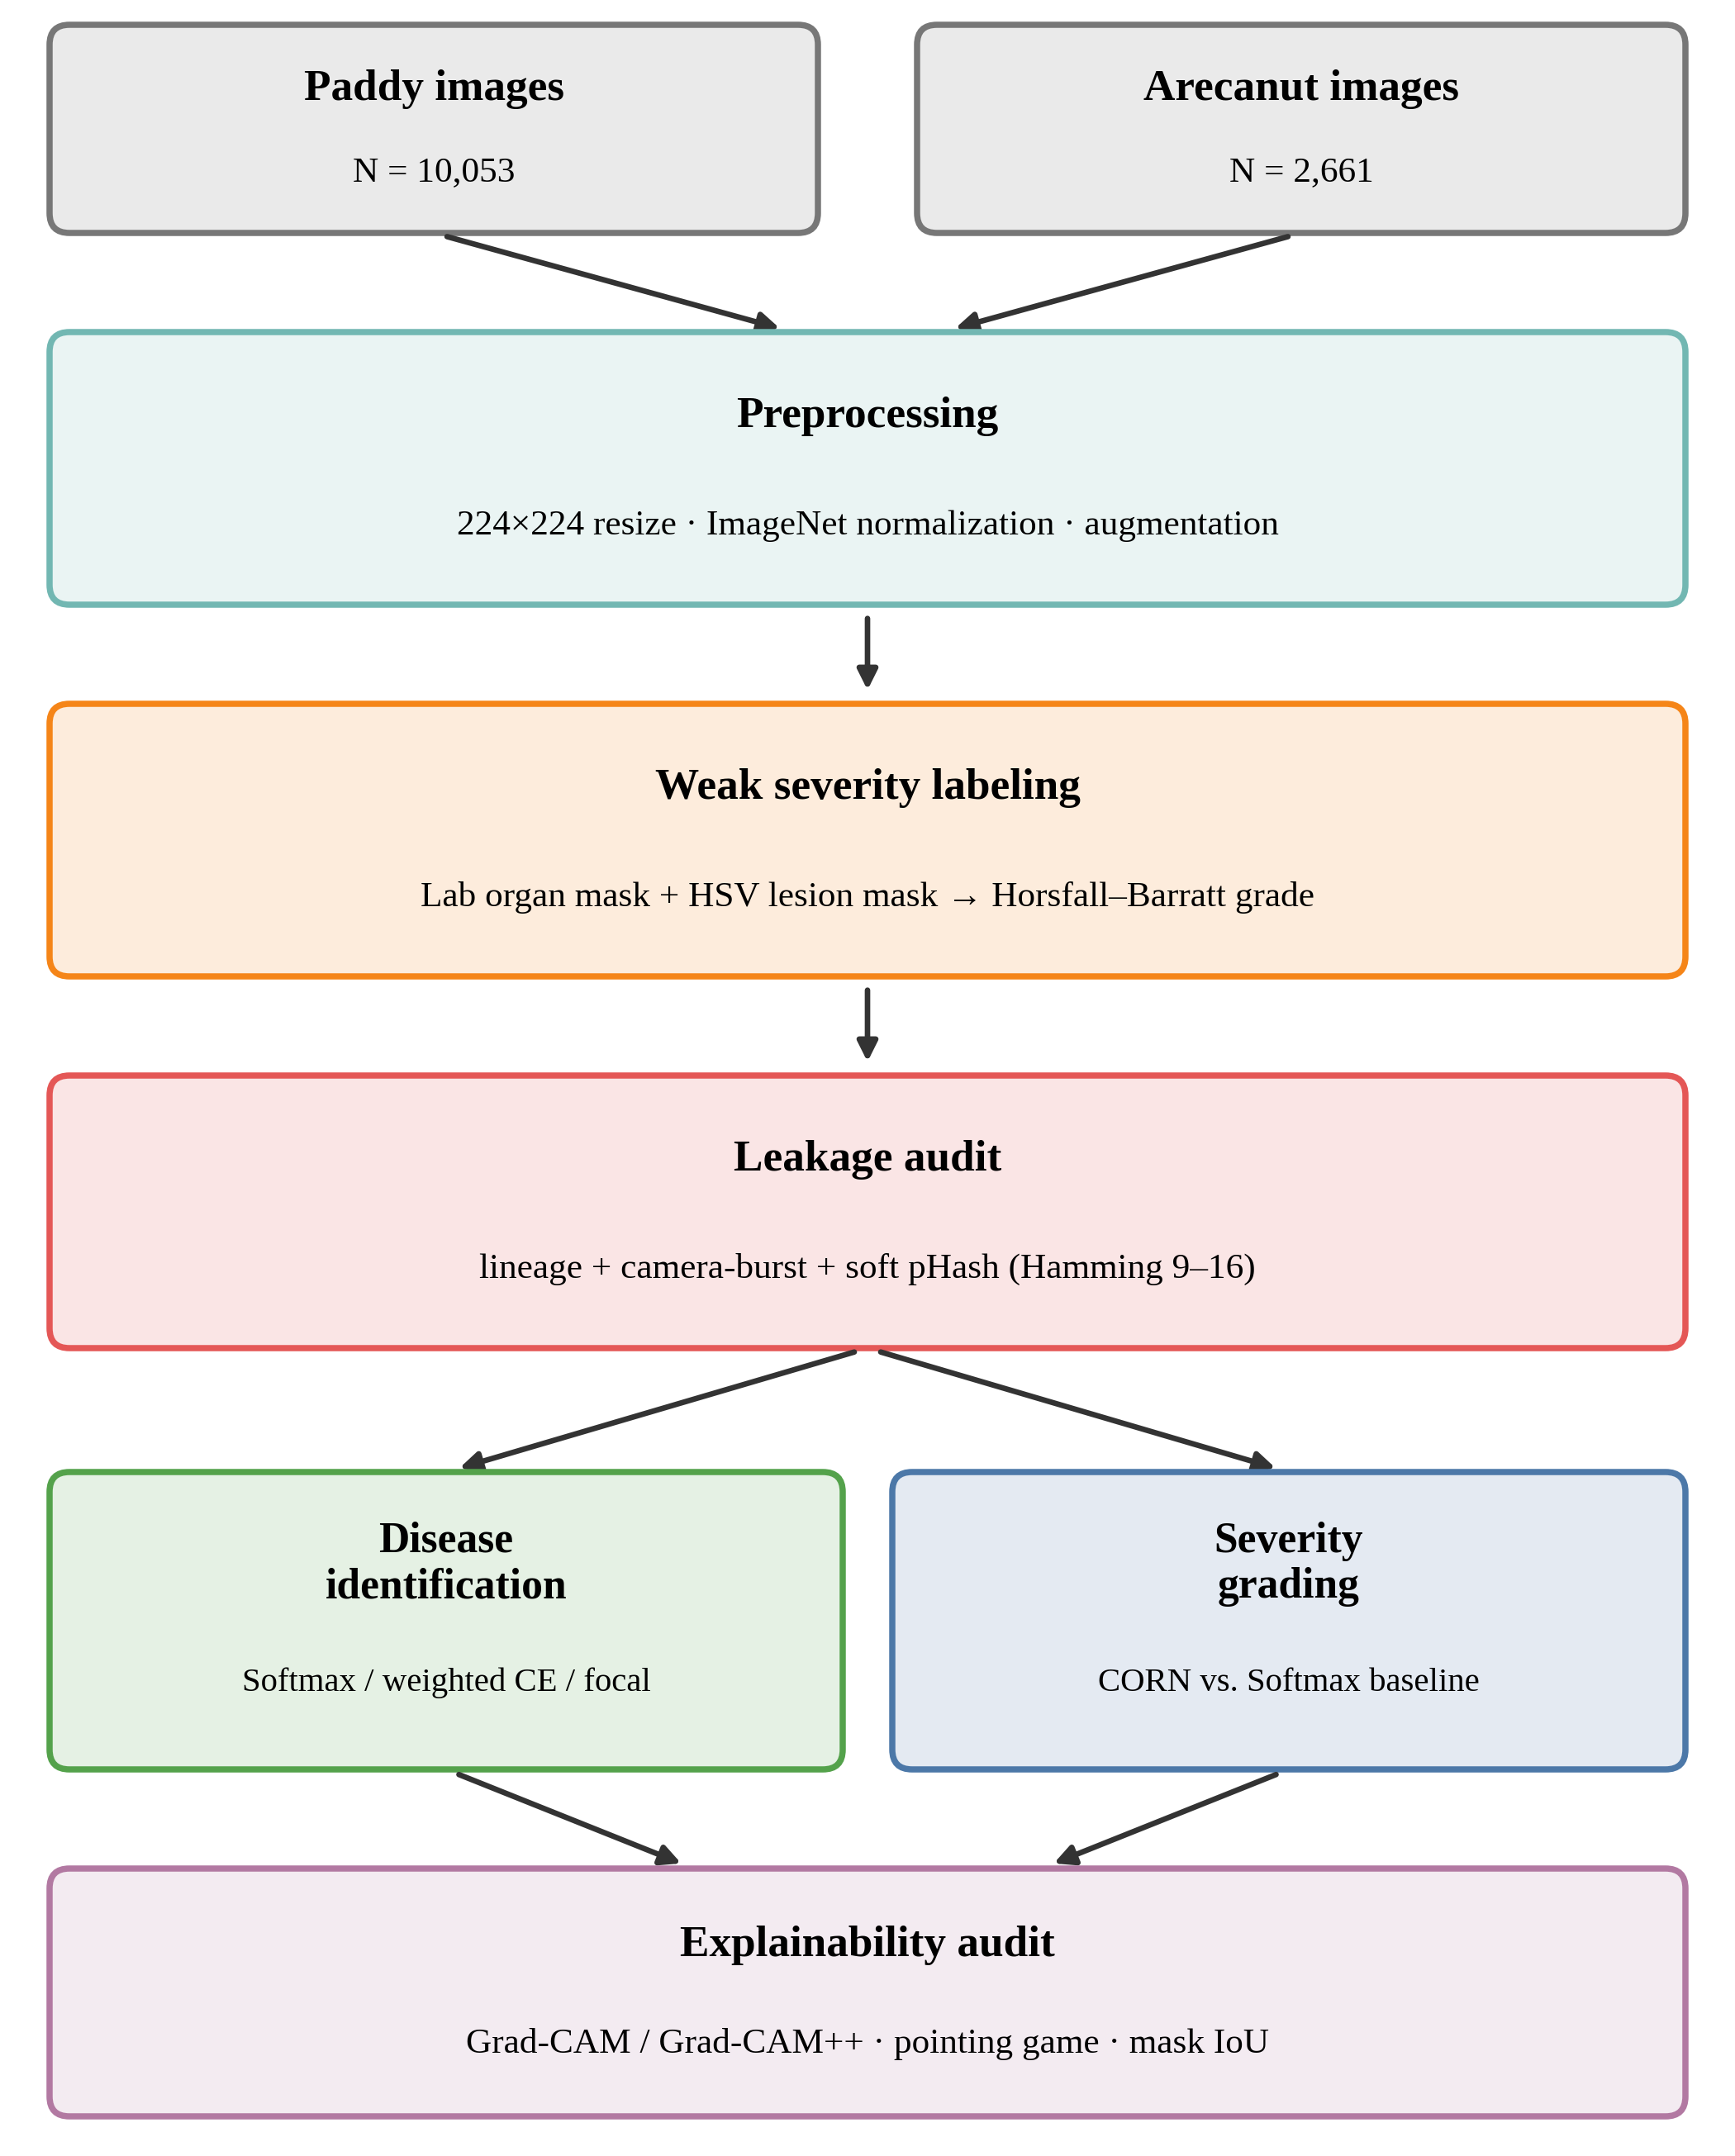
\includegraphics[width=\columnwidth]{figures/fig_process_pipeline.png}
\caption{End-to-end pipeline for weakly supervised, leakage-audited ordinal severity grading and disease identification across Paddy and Arecanut.}
\label{fig:process_pipeline}
\end{figure}

\section{Literature Review}

\subsection{Related Work}
Automated plant disease diagnosis has evolved from hand-crafted color/texture descriptors paired with classical classifiers toward end-to-end deep convolutional representations \cite{mohanty2016using, ferentinos2018deep}. Petchiammal et al. \cite{petchiammal2023paddy} introduced the Paddy Doctor dataset used in this work, a field-captured (rather than laboratory-controlled) benchmark across ten disease and healthy categories. For Arecanut, Kushalatha and Prasantha \cite{kushalatha2024spectroscopy} graded Crown-Choke disease severity using hyperspectral reflectance (250--2500\,nm) and gradient boosting, reaching high accuracy but requiring specialized hardware unsuitable for smallholder deployment. Neither prior Arecanut nor Paddy severity work in this space reports a split-leakage audit at the level of rigor applied here; this is a methodological gap our audit speaks to directly, independent of our own model's accuracy.

The Horsfall--Barratt scale \cite{horsfall1945fungicides} has long served as the standard framework for area-based severity grading, traditionally applied by trained human raters \cite{bock2022plant}. CORN \cite{shi2021corn}, building on rank-consistent ordinal regression \cite{cao2020rank}, decomposes a $K$-class ordinal problem into $K-1$ conditional binary sub-tasks trained only on the subset of samples with a given true rank, guaranteeing rank-monotonic predictions by construction. Grad-CAM \cite{selvaraju2017grad} and its higher-order extension Grad-CAM++ \cite{chattopadhay2018gradcampp} are the standard post-hoc attribution methods used in this literature, typically reported as a single illustrative heatmap rather than a quantitative, dataset-level localization audit, a gap we address in Section~V.

\subsection{Comparison with Prior Approaches}
Table~\ref{tab:literature_comp} compares our framework with representative prior work along key audit dimensions.

\begin{table}[htbp]
\caption{Comparison with Prior Crop Assessment Frameworks}
\centering
\resizebox{\columnwidth}{!}{%
\begin{tabular}{lcccc}
\toprule
\textbf{Audit Aspect} & \textbf{Petchiammal \cite{petchiammal2023paddy}} & \textbf{Kushalatha \cite{kushalatha2024spectroscopy}} & \textbf{Mohanty \cite{mohanty2016using}} & \textbf{Proposed} \\
\midrule
Split audit & MD5 only & Not reported & Random & Multi-criteria \\
Leakage check & Exact dup. & Not reported & Not reported & Soft-pHash \\
Explainability & None & Feature importance & None & Grad-CAM/++\,+\,IoU \\
\bottomrule
\end{tabular}%
}
\label{tab:literature_comp}
\end{table}

Unlike prior work, we apply a wider leakage check than exact-duplicate hashing, and we report the consequence of that wider check -- a substantial downward revision of our own initially reported Arecanut severity numbers -- rather than suppressing the uninflated figures.

\section{Dataset Description}

\subsection{Paddy Doctor Dataset (\textit{Oryza sativa})}
Sourced from the public Paddy Doctor benchmark \cite{petchiammal2023paddy}. After weakly supervised labeling and confidence filtering (Section~IV-B), 10,053 of the original 10,407 images were retained (96.60\%) and split 7,036 train / 1,510 validation / 1,507 test. The ten classes are: Bacterial Leaf Blight, Bacterial Leaf Streak, Bacterial Panicle Blight, Blast, Brown Spot, Dead Heart, Downy Mildew, Hispa, Normal (healthy), and Tungro. \texttt{Hispa} and \texttt{Dead Heart} are assigned fixed severity grades via domain fallback rules (Section~IV-B), and \texttt{Normal} is definitionally Grade 0; together these three classes account for 750 of 1,507 test images (49.8\%), a fact that materially affects how the full-test-set QWK should be interpreted (Section~V-A).

\subsection{Arecanut Dataset (\textit{Areca catechu})}
Field images collected across plantation sites in Karnataka, India, supplemented with a public Kaggle collection sharing the same two-day (August 19--20, 2023) photography campaign. After removing confirmed stock-photo/studio-image contamination and near-duplicate images, the clean pool used for disease identification contains 2,661 images (1,628 train / 547 validation / 486 test), spanning nine classes: \texttt{bud\_borer}, \texttt{healthy\_foot}, \texttt{healthy\_leaf}, \texttt{healthy\_nut}, \texttt{healthy\_trunk}, \texttt{mahali\_koleroga}, \texttt{stem\_bleeding}, \texttt{stem\_cracking}, and \texttt{yellow\_leaf\_disease} (YLD). As detailed in Section~IV-D, this pool derives from a small number of underlying physical trees and photography bursts, which materially limits how large a genuinely independent severity-grading test set can be constructed from it (Section~V-C).

\subsection{Weakly Supervised Severity Labeling}
Severity labels are derived from an adaptive dual-color-space segmentation pipeline. The organ boundary mask $\mathcal{M}_{\text{organ}}$ is extracted in Lab color space via adaptive Otsu thresholding; lesion pixels $\mathcal{M}_{\text{lesion}}$ are detected in HSV space. The lesion-area ratio is
\begin{equation}
\rho = \frac{\sum_{(x,y)} \mathcal{M}_{\text{lesion}}(x,y)}{\sum_{(x,y)} \mathcal{M}_{\text{organ}}(x,y)} \times 100\%,
\label{eq:ratio}
\end{equation}
discretized into Horsfall--Barratt grades:
\begin{equation}
y = \begin{cases}
0 \text{ (Healthy)}, & \rho = 0\% \\
1 \text{ (Mild)}, & 0\% < \rho \le 5\% \\
2 \text{ (Moderate)}, & 5\% < \rho \le 15\% \\
3 \text{ (Severe)}, & \rho > 15\%.
\end{cases}
\label{eq:hb_scale}
\end{equation}
A composite confidence filter routes ambiguous boundary cases to human review (3.40\% of Paddy images). Two Paddy classes use domain-expert fallback rules rather than this pipeline: \texttt{Hispa} (texture-based scrape streaks overcounted lesion area; fixed to Grade~1) and \texttt{Dead Heart} (stem-borer apical mortality, not distributed spotting; fixed to Grade~3). For Arecanut, \texttt{yellow\_leaf\_disease} (YLD) causes diffuse whole-frond chlorosis rather than discrete necrotic spots, which this area-ratio pipeline cannot correctly stage; we therefore exclude YLD from severity-grading evaluation (though it remains part of disease identification), affecting 86 test images.

We note explicitly that this same labeling pipeline is used as the ground truth against which our explainability audit (Section~V-D) is later compared; we return to this circularity in Section~VI.

\subsection{Split Construction and the Discovery of Soft-Lineage Leakage}
\label{sec:leakage}
Paddy images were deduplicated by MD5 and perceptual hashing (pHash, Hamming $\le 5$) prior to a stratified 70/15/15 split. A subsequent audit at a wider threshold (Hamming $\le 8$) found that 775 of 1,507 Paddy test images (51.4\%) still had a near-duplicate twin in train or validation; we report both the full and twin-adjusted results in Section~V-A.

For Arecanut, we iteratively constructed four different train/test splits over the course of this work, each intended to be leak-free, using progressively stricter criteria: (i) an initial 124-image pilot split using parent-plant timestamp grouping; (ii) a 146-image split adding perceptual-hash deduplication; (iii) a 502-image split expanding the training pool with external Kaggle images filtered by exact-duplicate pHash (Hamming $\le 8$); and (iv) a 486-image split built using connected-component clustering over base-photo IDs, camera-burst windows ($\le 120$\,s), and pHash (Hamming $\le 5$), which we initially reported, and briefly published a draft of this manuscript around, as 100\% leak-free.

A subsequent audit applying a \emph{soft} perceptual-hash threshold (Hamming distance 9--16, i.e., images that are visually similar but not exact or near-exact duplicates) found that every one of these four splits exhibited substantial train/test overlap by this wider criterion, even though each had passed its narrower, exact-duplicate-oriented check:

\begin{table}[htbp]
\caption{Session-Level Overlap Found by Widening the Leakage Check}
\centering\footnotesize
\begin{tabular}{lcc}
\toprule
\textbf{Split ($N_{\text{test}}$)} & \textbf{Passed narrow check?} & \textbf{Wide-check overlap} \\
\midrule
124-image pilot & Yes (0\% reported) & 71.8\% (89/124) \\
146-image & Yes (0\% reported) & 76.7\% (112/146) \\
502-image (expanded) & Yes (0\% reported) & 77.9\% (391/502) \\
486-image (``v2'') & Yes (0\% reported) & 80.5\% (391/486) \\
\bottomrule
\end{tabular}
\label{tab:leakage_discovery}
\end{table}

The overlap is driven by same-session photography: images of the same tree, taken seconds to minutes apart under near-identical lighting and background, differ enough in crop, rotation, or exposure to evade exact-duplicate detection, while remaining visually recognizable to a trained CNN. We find this pattern consistently across every Arecanut split attempted in this work, including ones we ourselves built and initially trusted, which we interpret as a structural property of the underlying photo collection (traceable to a small number of base photography sessions) rather than a flaw specific to any one clustering method. We report this discovery process in full because we believe the same failure mode is likely under-detected in other small, field-collected agricultural benchmarks evaluated only with exact-duplicate deduplication.

For each split, we identify the subset of test images with \emph{zero} overlap under the wide check (lineage, burst, and soft-pHash combined) and treat only that subset as a genuinely independent evaluation set. The largest such isolated subset available in this work is $N=111$ (39 independent clusters), drawn from split (iii); results on this subset are reported as our primary Arecanut severity finding in Section~V-C.

\section{Methodology}

\subsection{Proposed Framework}
Fig.~\ref{fig:process_pipeline} illustrates the complete pipeline: weakly supervised labeling (Section~III-C), leakage-audited splitting (Section~III-D), deep ordinal/nominal classification (Section~IV-C), explainability auditing (Section~V-D), and a lightweight MobileNetV2 deployment path.

\subsection{Preprocessing}
Images are resized to $224\times224$ and normalized to ImageNet statistics. Training-time augmentation (random rotation $\pm30^\circ$, horizontal/vertical flip, color jitter) is applied identically to both crops; validation and test images are not augmented.

\subsection{Models}
We evaluate ResNet-18 (11.2M parameters), ResNet-34 (21.8M) \cite{he2016deep}, and MobileNetV2 (2.2M) \cite{sandler2018mobilenetv2} backbones, each with ImageNet-pretrained weights. For disease identification, a standard Softmax (Paddy) or class-weighted / focal-loss \cite{lin2017focal} (Arecanut) head is used. For severity grading, we compare the CORN ordinal head against a Softmax baseline.

CORN outputs $K-1=3$ logits, each a conditional binary sub-task trained only on the subset $S_j=\{i:y_i\ge j\}$:
\begin{equation}
\sigma(f_j(\mathbf{x})) = P(y>j \mid y\ge j, \mathbf{x}), \quad j\in\{0,1,2\}.
\end{equation}
Unconditional rank probabilities follow the chain rule,
\begin{equation}
P(y>j\mid\mathbf{x}) = \prod_{k=0}^{j}\sigma(f_k(\mathbf{x})),
\label{eq:chain}
\end{equation}
which is non-increasing in $j$ by construction. The predicted grade is decoded as the class with maximum probability mass under this chain, $\hat{y} = \arg\max_k P(y=k\mid\mathbf{x})$, where $P(y=k\mid\mathbf{x}) = P(y>k-1\mid\mathbf{x}) - P(y>k\mid\mathbf{x})$; we selected this decode rule, rather than the simpler threshold-sum rule sometimes used in the literature, because it gave the highest validation QWK among three candidate decode rules tested, and we report this selection explicitly because we found the choice of decode rule to materially affect reported results (a discrepancy we traced and corrected during this work).

\subsection{Explainability Audit}
We audit model attention with both Grad-CAM \cite{selvaraju2017grad} and Grad-CAM++ \cite{chattopadhay2018gradcampp} at the final convolutional layer. Heatmaps are binarized at threshold $T=0.5$ and compared to the lesion mask $\mathcal{M}_{\text{lesion}}$ via Intersection-over-Union,
\begin{equation}
\text{IoU} = \frac{|\mathcal{B}_{\text{Grad-CAM}} \cap \mathcal{M}_{\text{lesion}}|}{|\mathcal{B}_{\text{Grad-CAM}} \cup \mathcal{M}_{\text{lesion}}|},
\end{equation}
and via a pointing-game test of whether the single maximum-activation pixel falls inside the lesion mask, evaluated on diseased samples only.

\subsection{Experimental Setup}
Models were trained with AdamW (learning rate $10^{-4}$, weight decay $10^{-4}$), batch size 16, with early stopping on validation QWK. Evaluation uses QWK \cite{cohen1968weighted}, MAE, Exact Match Accuracy, Within-1-Grade Accuracy, and Macro-F1. Statistical comparisons use McNemar's paired test \cite{mcnemar1947note} on exact-match correctness and parent/cluster-grouped bootstrap resampling (2,000 iterations) for confidence intervals, grouping by the same physical-entity clusters used for split construction so that resampled observations respect the same independence structure as the splits themselves.

\section{Results}

\subsection{Paddy: Disease Identification and Severity Grading}
Our ResNet-18 disease classifier reaches 96.04\% accuracy on the twin-free test subset ($N=732$, Hamming $\le 8$). A two-class healthy/diseased screening model reaches 98.36\% [97.40, 99.18]\% accuracy on the same subset.

For severity grading, Table~\ref{tab:paddy_severity} reports CORN's QWK on progressively stricter evaluation subsets. The full-test-set QWK of 0.9390 is substantially inflated by the three class-determined categories noted in Section~III-A (Normal, Hispa, Dead Heart, 49.8\% of the test set) and by near-duplicate test images; restricting to the seven genuinely lesion-graded classes and removing twins drops QWK to 0.56--0.71 depending on the duplicate threshold applied. We report the full-test number because it is the quantity most comparable to prior literature, but we consider the lesion-only, twin-free number the more meaningful estimate of genuine severity-grading skill.

\begin{table}[htbp]
\caption{Paddy CORN Severity QWK Under Progressively Stricter Evaluation}
\centering\footnotesize
\begin{tabular}{lcc}
\toprule
\textbf{Evaluation subset} & \textbf{$N$} & \textbf{QWK} \\
\midrule
Full test set & 1,507 & 0.9390 \\
Lesion classes only & 757 & 0.7126 \\
Lesion classes, twin-free (Hamming $\le 8$) & 343 & 0.7055 [0.589, 0.800] \\
\bottomrule
\end{tabular}
\label{tab:paddy_severity}
\end{table}

\begin{figure}[htbp]
\centering
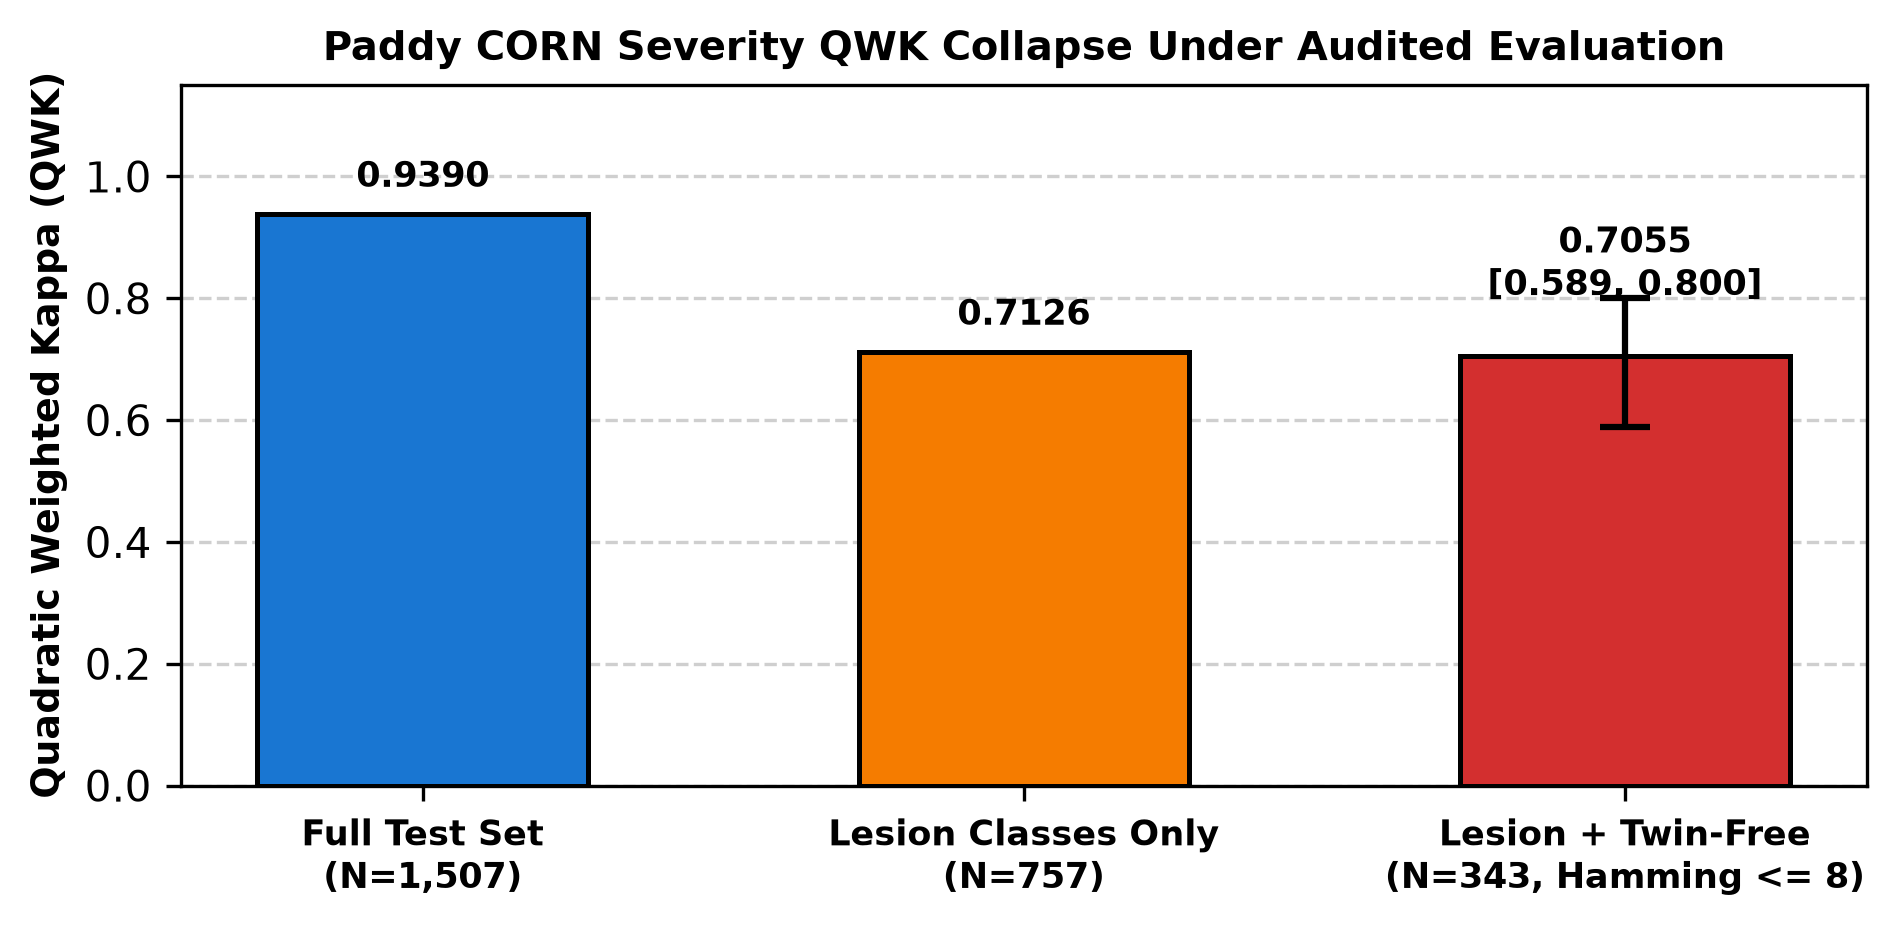
\includegraphics[width=\columnwidth]{figures/fig6_qwk_progression.png}
\caption{Progression of Paddy severity QWK as class-determined categories (Normal, Hispa, Dead Heart) and near-duplicate twins ($\text{Hamming} \le 8$) are removed ($0.9390 \rightarrow 0.7126 \rightarrow 0.7055$). Error bar indicates 95\% bootstrap confidence interval [0.589, 0.800] for the twin-free subset.}
\label{fig:qwk_progression}
\end{figure}

McNemar's test on exact-match correctness between CORN and Softmax shows no statistically significant difference ($p=0.656$), consistent with the theoretical role of the ordinal loss: on the full test set, severe reversals ($|\Delta|\ge2$) account for only 18 of 1,507 predictions (1.19\%) under CORN, with the great majority of errors confined to adjacent-grade confusion.

\subsection{Class-Only Baseline: Severity Metrics Confounded with Disease Identity}
A trivial baseline that ignores the input image and predicts each test image's grade as the most common training-set grade for its disease class achieves QWK $\ge 0.91$ on several Arecanut evaluation subsets we examined, exceeding several of our own trained CORN and Softmax severity models. This arises because many Arecanut disease classes are strongly or entirely associated with a single severity grade in available data (e.g., \texttt{bud\_borer} is overwhelmingly Grade 3; several healthy-tissue classes are definitionally Grade 0), so a model, or a naive baseline, can achieve a high aggregate QWK by recognizing \emph{which disease} is present rather than assessing \emph{how severe} it is. On Paddy, the class-only baseline reaches QWK $\approx 0.91$ on the full test set but only $0.00$ on the lesion-only subset (by construction, since within a single class there is no majority grade to exploit), confirming that the lesion-only evaluation in Table~\ref{tab:paddy_severity} is the subset where genuine severity discrimination is actually being tested. We report this finding because, absent this check, a high aggregate QWK could be mistaken for severity-grading skill when it is substantially explained by disease recognition.

\subsection{Arecanut Severity Grading on the Audited, Isolated Test Subset}
As established in Section~III-D, we do not consider any of our four constructed Arecanut splits leak-free by the wide (soft-pHash) criterion, including the 486-image split we initially reported as such. We therefore report Arecanut severity results only on the isolated subsets with zero session-level overlap under all three criteria.

On the largest such subset ($N=111$, 39 independent physical clusters, drawn from split (iii) in Table~\ref{tab:leakage_discovery}), three-seed CORN achieves QWK $=0.6998\pm0.0449$ versus Softmax QWK $=0.6280\pm0.1039$ (Table~\ref{tab:areca_severity}). A smaller, preliminary isolated subset ($N=34$, from split (ii)) yielded a directionally consistent result for ResNet-18 (QWK $\approx 0.69$), but with single-digit counts across intermediate grades, it remains noise-dominated and is omitted as a standalone point estimate.

\begin{table}[htbp]
\caption{Arecanut Severity Grading on the Audited Isolated Test Subset ($N=111$)}
\centering\footnotesize
\begin{tabular}{lccc}
\toprule
\textbf{Model} & \textbf{QWK (3-seed)} & \textbf{Exact Acc.} & \textbf{MAE} \\
\midrule
CORN (ResNet-18) & $0.6998 \pm 0.0449$ & 78.98\% & 0.487 \\
Softmax (ResNet-18) & $0.6280 \pm 0.1039$ & 72.97\% & 0.604 \\
\bottomrule
\end{tabular}
\label{tab:areca_severity}
\end{table}

The bootstrap confidence intervals for individual seeds on this subset are wide (e.g., [0.41, 0.98] for CORN, seed-dependent), reflecting both the small sample size and severe grade imbalance: Grades 1 and 2 together comprise only 7 of the 111 images. We therefore do not claim a statistically significant CORN-over-Softmax advantage at this sample size; the point estimates are directionally consistent with CORN's rank-consistency property but the intervals overlap. We report both numbers, with their uncertainty, rather than either number alone.

\begin{table}[htbp]
\caption{Arecanut Disease Identification (Twin-Checked Test Set, $N=486$)}
\centering\footnotesize
\resizebox{\columnwidth}{!}{%
\begin{tabular}{lcc}
\toprule
\textbf{Model} & \textbf{Accuracy [95\% CI]} & \textbf{Macro-F1 [95\% CI]} \\
\midrule
Focal loss (baseline) & 82.92\% [72.82, 91.88] & 73.05\% [59.46, 83.09] \\
Cross-entropy + weights & 90.33\% [83.55, 96.19] & 85.13\% [71.52, 91.35] \\
\bottomrule
\end{tabular}%
}
\label{tab:areca_disease}
\end{table}

Table~\ref{tab:areca_disease} reports disease identification on the twin-checked (Hamming $\le 8$) 486-image test set. The two loss configurations' confidence intervals overlap by 8.33 percentage points, so the apparent 7.4-point accuracy gap is not statistically distinguishable at this sample size. We note that minority-class \texttt{bud\_borer} recall remains at 0.0\% (0/33) across both loss configurations on the clean twin-checked test set, demonstrating a data scarcity bottleneck as this class derives from only five distinct base photo lineages in the available data.

\subsection{Explainability Audit}
Fig.~\ref{fig:explainability} shows Grad-CAM IoU plotted against ground-truth lesion coverage across eight Paddy classes, confirming a strong linear relationship ($R^2=0.82$): apparent localization quality is substantially explained by how much of the image a class's lesion happens to cover, rather than by true localization precision.

\begin{figure}[htbp]
\centering
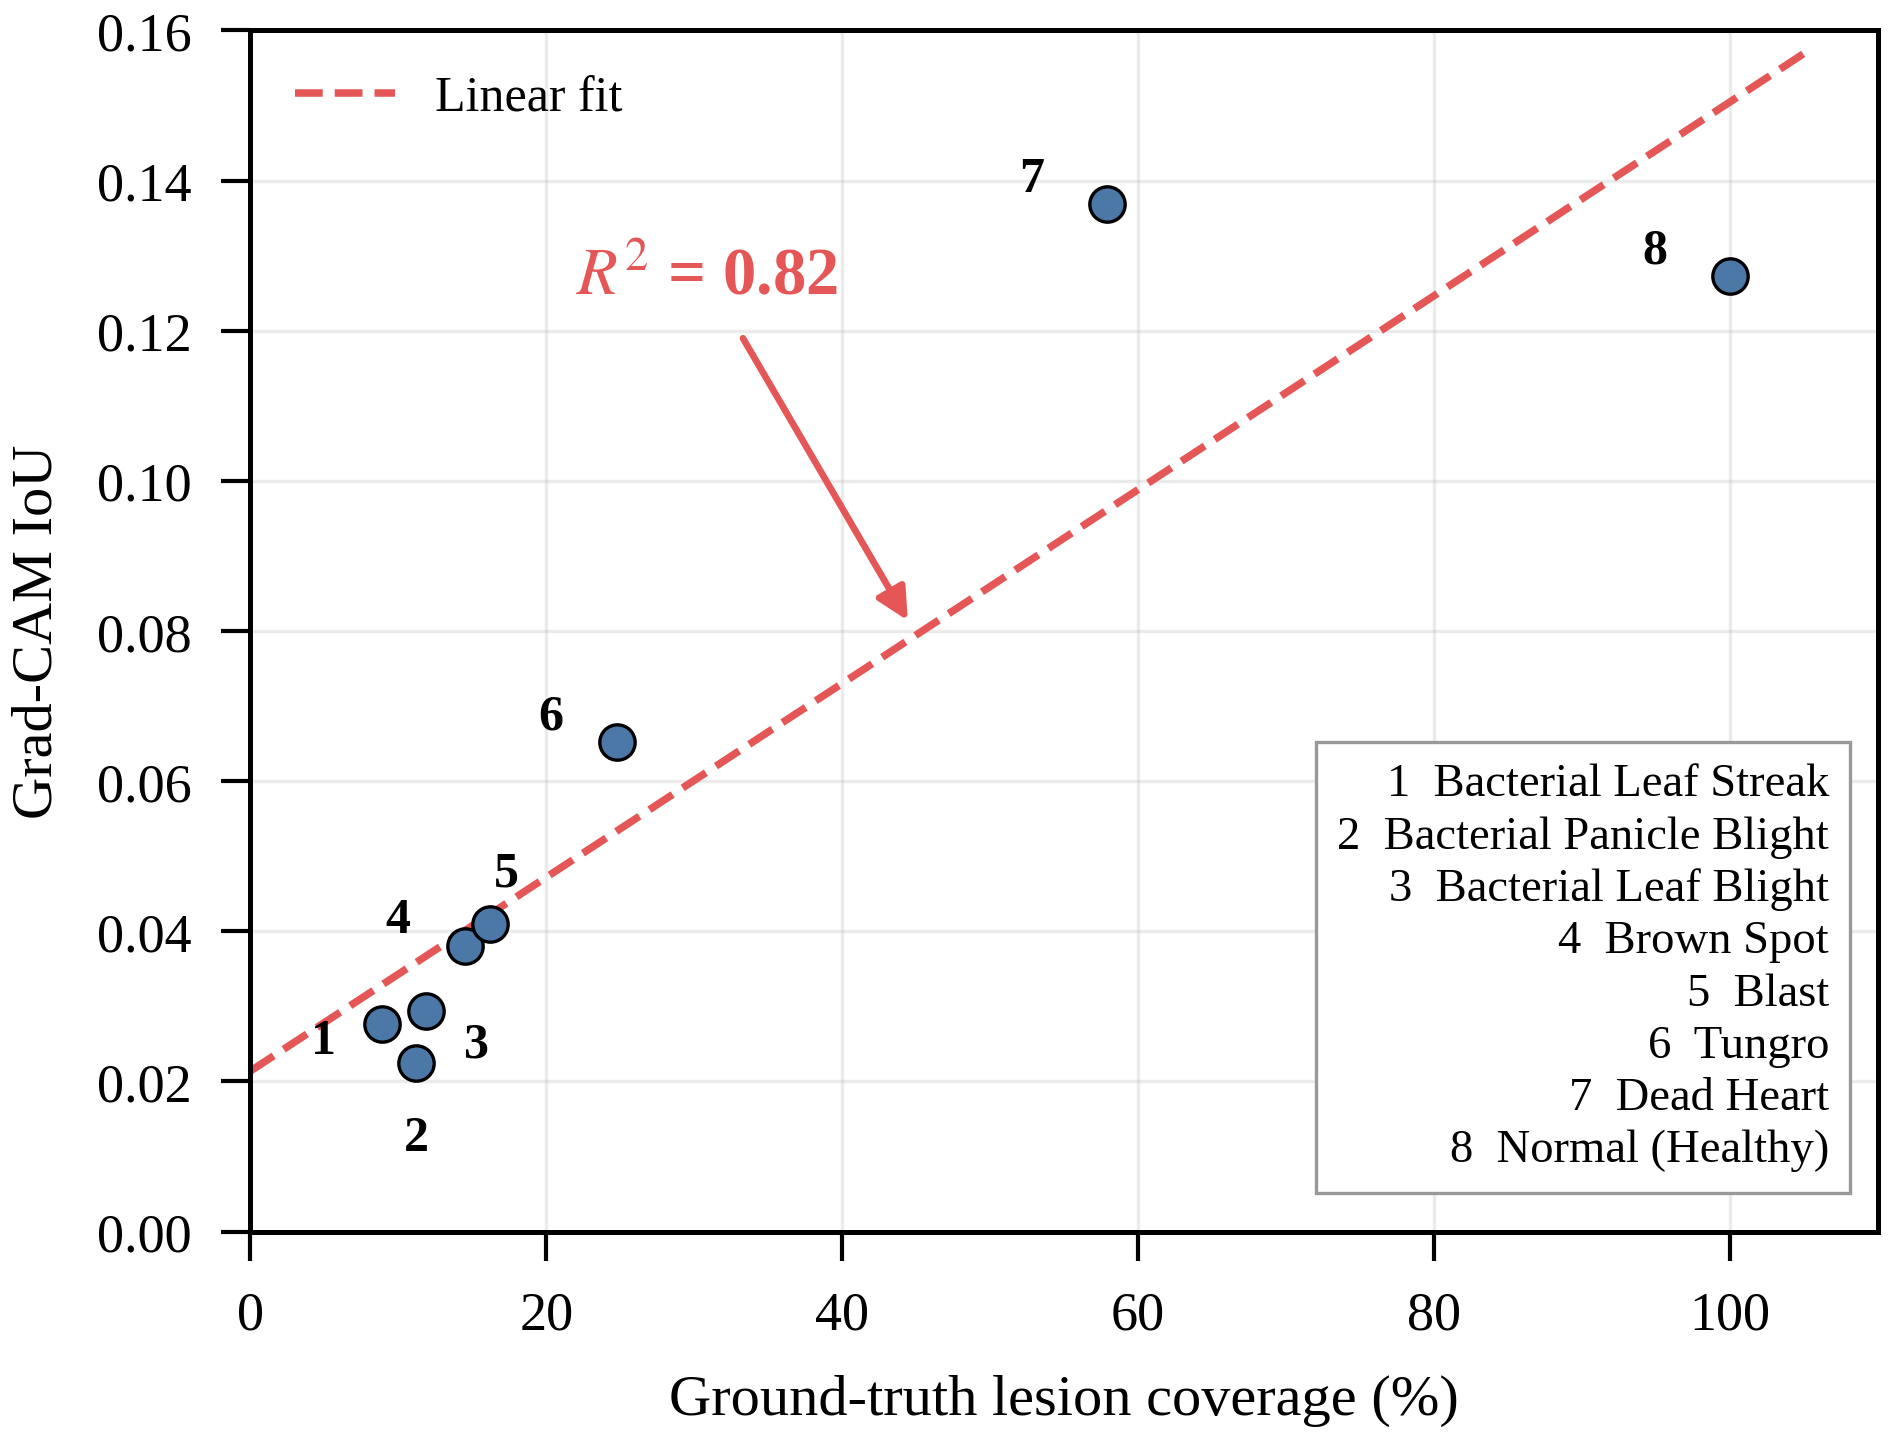
\includegraphics[width=\columnwidth]{figures/fig_iou_confound.png}
\caption{Grad-CAM IoU versus ground-truth lesion coverage, Paddy classes ($R^2=0.82$). Numbers index classes: 1~Bacterial Leaf Streak, 2~Bacterial Panicle Blight, 3~Bacterial Leaf Blight, 4~Brown Spot, 5~Blast, 6~Tungro, 7~Dead Heart, 8~Normal.}
\label{fig:explainability}
\end{figure}

Diseased-tissue pointing-game accuracy, computed with both Grad-CAM and Grad-CAM++, is 13.9\%/11.4\% on Paddy and 4.6\%/4.6\% on Arecanut; several disease classes score exactly 0\% under both methods. Because two attribution methods with different underlying mechanisms converge on the same near-zero localization rate, we conclude this reflects a genuine property of the learned representation -- substantial reliance on non-lesion visual cues -- rather than an artifact of either attribution method.

Fig.~\ref{fig:confusion_matrices} shows confusion matrices for the primary configurations discussed above.

\begin{figure}[htbp]
\centering
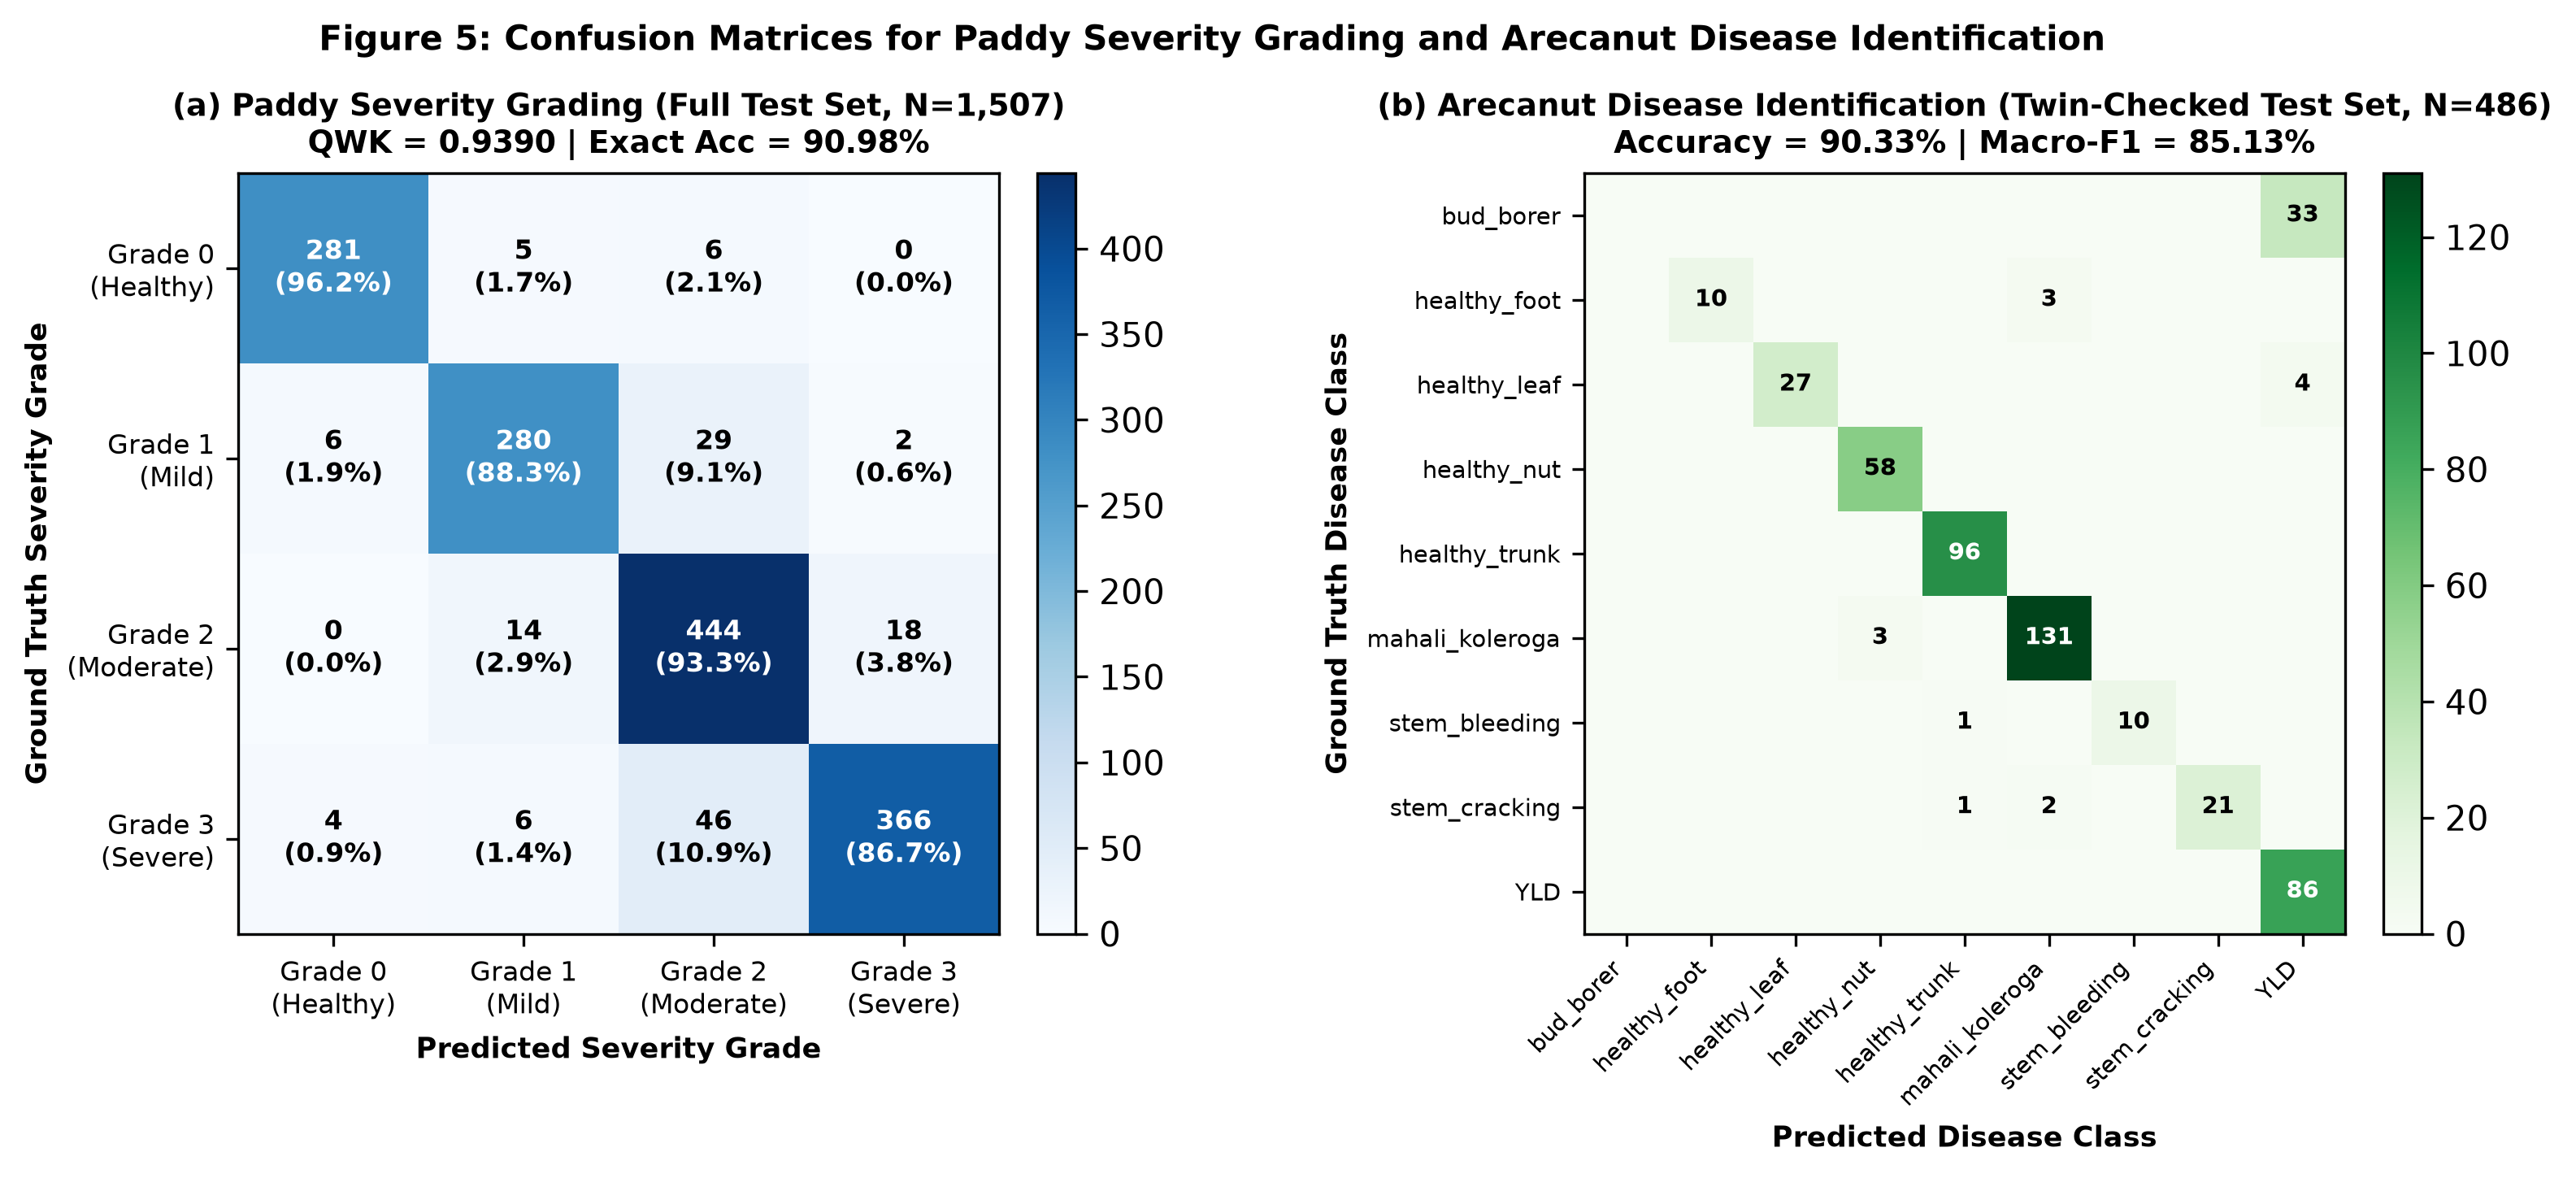
\includegraphics[width=\columnwidth]{figures/fig_confusion_matrices.png}
\caption{Confusion matrices for primary model configurations. (a)~Paddy full test set severity grading (ResNet-18, CORN, $N=1{,}507$, QWK = 0.9390). (b)~Arecanut 9-class disease identification on the twin-checked test set (ResNet-18, cross-entropy + class weights, $N=486$, accuracy = 90.33\%).}
\label{fig:confusion_matrices}
\end{figure}

\section{Discussion and Limitations}
\begin{enumerate}
    \item \textbf{Auto-labeling circularity}: our severity labels, and the lesion masks used in the explainability audit, derive from the same color-threshold pipeline (Eqs.~\ref{eq:ratio}--\ref{eq:hb_scale}). A model that learns to imitate this heuristic would score well on both the severity task and a mask-based IoU audit without having learned true pathology. The pointing-game audit (Section~V-D) partially probes this, since pointing accuracy is low even on this same self-referential ground truth, but an independent human-graded validation set remains necessary before these labels can be treated as ground truth in a stronger sense.
    \item \textbf{YLD and lesion-ratio mismatch}: diffuse chlorosis is not well modeled by a local lesion-area ratio; we exclude YLD from severity evaluation rather than report a staging we do not trust.
    \item \textbf{Arecanut severity sample size is small and imbalanced}: the largest fully audited, isolated Arecanut severity test set available in this work is $N=111$, with only 7 images across the two intermediate grades. This limits the statistical power of any Arecanut severity comparison, including the CORN-vs-Softmax comparison reported here, and should be treated as a preliminary estimate pending a larger, independently collected dataset.
    \item \textbf{Bud borer recall and dataset expansion}: An initial training expansion using external images appeared to recover \texttt{bud\_borer} recall from 0.0\% (0/33) to 33.3\% (11/33), but a soft-pHash lineage audit revealed that 100\% of the correctly predicted test samples shared near-duplicate photo lineages ($\text{Hamming} \le 16$) with the added training set. Discarding the leaky external samples restored true, clean recall to 0.0\% (0/33).
    \item \textbf{Single-campaign collection window}: available Arecanut photography, including the external data we incorporated, derives from a two-day collection window (August 19--20, 2023) at specific plantation sites, limiting seasonal and geographic generalization. We note this is also a likely structural cause of the lineage-overlap problem documented in Section~III-D: a narrow collection window produces a small pool of underlying physical trees, which splitting algorithms cannot fully compensate for.
    \item \textbf{Class-identity confound}: Section~V-B shows that headline severity QWK on Arecanut is confounded with disease identity. Any future reporting of Arecanut severity results, by us or others, should include the class-only baseline alongside the trained model's result.
    \item \textbf{Unverified components}: the out-of-distribution ``gatekeeper'' screening model used in our deployed demonstration application was validated only against a convenience set of non-agricultural desktop images, not a curated real-world out-of-domain benchmark, and we do not report it as a measured result. A prepared, blinded human-grading instrument for independent severity validation exists but had not been completed by the time of writing; we report its design and intended use as future work rather than results.
\end{enumerate}

\section{Conclusion}
We presented an explainable framework for joint disease identification and ordinal severity grading on Paddy and Arecanut, and subjected every stage, not only the final accuracy numbers, to independent statistical and leakage verification. Paddy results are comparatively robust: 96.04\% disease-identification accuracy and a genuine lesion-only severity QWK of 0.71, with no statistically significant difference between CORN and Softmax losses. Arecanut results required substantially more scrutiny: an initial, seemingly leak-free split and its corresponding QWK of 0.87 did not survive a wider soft-perceptual-hash audit, which found 70--80\% train/test session overlap across every split we constructed over the course of this work. On the most rigorously isolated Arecanut subset we could establish, genuine severity-grading skill is modest (QWK $\approx 0.70$) and not yet distinguishable between loss functions at the available sample size. A class-only baseline further shows that headline severity metrics on this crop are confounded with disease recognition. We report these negative and null findings alongside the positive ones because we believe the leakage-discovery process itself -- including the fact that our own initial audit was insufficient and required a second, wider pass to catch -- is a transferable methodological contribution for a field where small, field-collected datasets with repeated photography sessions are common and leakage audits are not yet standard practice.

\section*{Acknowledgment}
The author thanks the open-source contributors of the Paddy Doctor benchmark and the plantation sites in Karnataka, India, that supported Arecanut field data collection.

\begin{thebibliography}{00}
\bibitem{petchiammal2023paddy}
P.~Petchiammal, D.~Murugan, and P.~Shanmuga~Sundaram, ``Paddy doctor: A large-scale benchmark dataset for visual disease classification in paddy,'' in \emph{Proc. 6th Joint Int. Conf. Data Sci. Manage. Data (CODS-COMAD)}, 2023, pp. 317--321.

\bibitem{mohanty2016using}
S.~P. Mohanty, D.~P. Hughes, and M.~Salath{\'e}, ``Using deep learning for image-based plant disease detection,'' \emph{Front. Plant Sci.}, vol.~7, p. 1419, 2016.

\bibitem{ferentinos2018deep}
K.~P. Ferentinos, ``Deep learning models for plant disease detection and diagnosis,'' \emph{Comput. Electron. Agric.}, vol. 145, pp. 311--318, 2018.

\bibitem{horsfall1945fungicides}
J.~G. Horsfall and R.~W. Barratt, ``An improved grading system for measuring plant diseases,'' \emph{Phytopathology}, vol.~35, no.~8, p. 655, 1945.

\bibitem{bock2022plant}
C.~H. Bock, K.~S. Chiang, and E.~M. Del~Ponte, ``Plant disease severity estimated visually: A review of the senses, scales and stories,'' \emph{Plant Pathol.}, vol.~71, no.~1, pp. 14--34, 2022.

\bibitem{kushalatha2024spectroscopy}
M.~Kushalatha and H.~S. Prasantha, ``Identification of arecanut disease severity using spectral reflectance signatures and machine learning algorithms,'' \emph{Spectrochim. Acta Part A Mol. Biomol. Spectrosc.}, vol. 306, p. 123594, 2024.

\bibitem{selvaraju2017grad}
R.~R. Selvaraju, M.~Cogswell, A.~Das, R.~Vedantam, D.~Parikh, and D.~Batra, ``Grad-CAM: Visual explanations from deep networks via gradient-based localization,'' in \emph{Proc. IEEE Int. Conf. Comput. Vis. (ICCV)}, 2017, pp. 618--626.

\bibitem{chattopadhay2018gradcampp}
A.~Chattopadhay, A.~Sarkar, P.~Howlader, and V.~N. Balasubramanian, ``Grad-CAM++: Generalized gradient-based visual explanations for deep convolutional networks,'' in \emph{Proc. IEEE Winter Conf. Appl. Comput. Vis. (WACV)}, 2018, pp. 839--847.

\bibitem{cao2020rank}
W.~Cao, V.~Mirjalili, and S.~Raschka, ``Rank consistent ordinal regression for neural networks with application to age estimation,'' \emph{Pattern Recognit. Lett.}, vol. 140, pp. 325--331, 2020.

\bibitem{shi2021corn}
X.~Shi, X.~Cao, and S.~Raschka, ``Deep neural networks for rank-consistent ordinal regression based on conditional probabilities,'' \emph{Pattern Recognit. Lett.}, vol. 152, pp. 10--16, 2021.

\bibitem{he2016deep}
K.~He, X.~Zhang, S.~Ren, and J.~Sun, ``Deep residual learning for image recognition,'' in \emph{Proc. IEEE Conf. Comput. Vis. Pattern Recognit. (CVPR)}, 2016, pp. 770--778.

\bibitem{sandler2018mobilenetv2}
M.~Sandler, A.~Howard, M.~Zhu, A.~Zhmoginov, and L.-C. Chen, ``MobileNetV2: Inverted residuals and linear bottlenecks,'' in \emph{Proc. IEEE Conf. Comput. Vis. Pattern Recognit. (CVPR)}, 2018, pp. 4510--4520.

\bibitem{lin2017focal}
T.-Y. Lin, P.~Goyal, R.~Girshick, K.~He, and P.~Doll{\'a}r, ``Focal loss for dense object detection,'' in \emph{Proc. IEEE Int. Conf. Comput. Vis. (ICCV)}, 2017, pp. 2980--2988.

\bibitem{cohen1968weighted}
J.~Cohen, ``Weighted kappa: Nominal scale agreement provision for scaled disagreement or partial credit,'' \emph{Psychol. Bull.}, vol.~70, no.~4, pp. 213--220, 1968.

\bibitem{mcnemar1947note}
Q.~McNemar, ``Note on the sampling error of the difference between correlated proportions or percentages,'' \emph{Psychometrika}, vol.~12, no.~2, pp. 153--157, 1947.
\end{thebibliography}

\end{document}
